\subsection{Подготовка данных для COLMAP}

Пайплайн 3DGS требует данных в формате COLMAP, поэтому чтобы встроить текущую работу в него, потребуется разобраться с внутренним устройством.

COLMAP и Blender это инструменты для работы с 3D из разных областей: первый относится к компьютерному зрению, а второй к компьютерной графике; из-за этого они оба устроены по разному с точки зрения систем координат. Софт обычно отличается по трем характеристикам.

\begin{figure}[htbp]
	\centering
	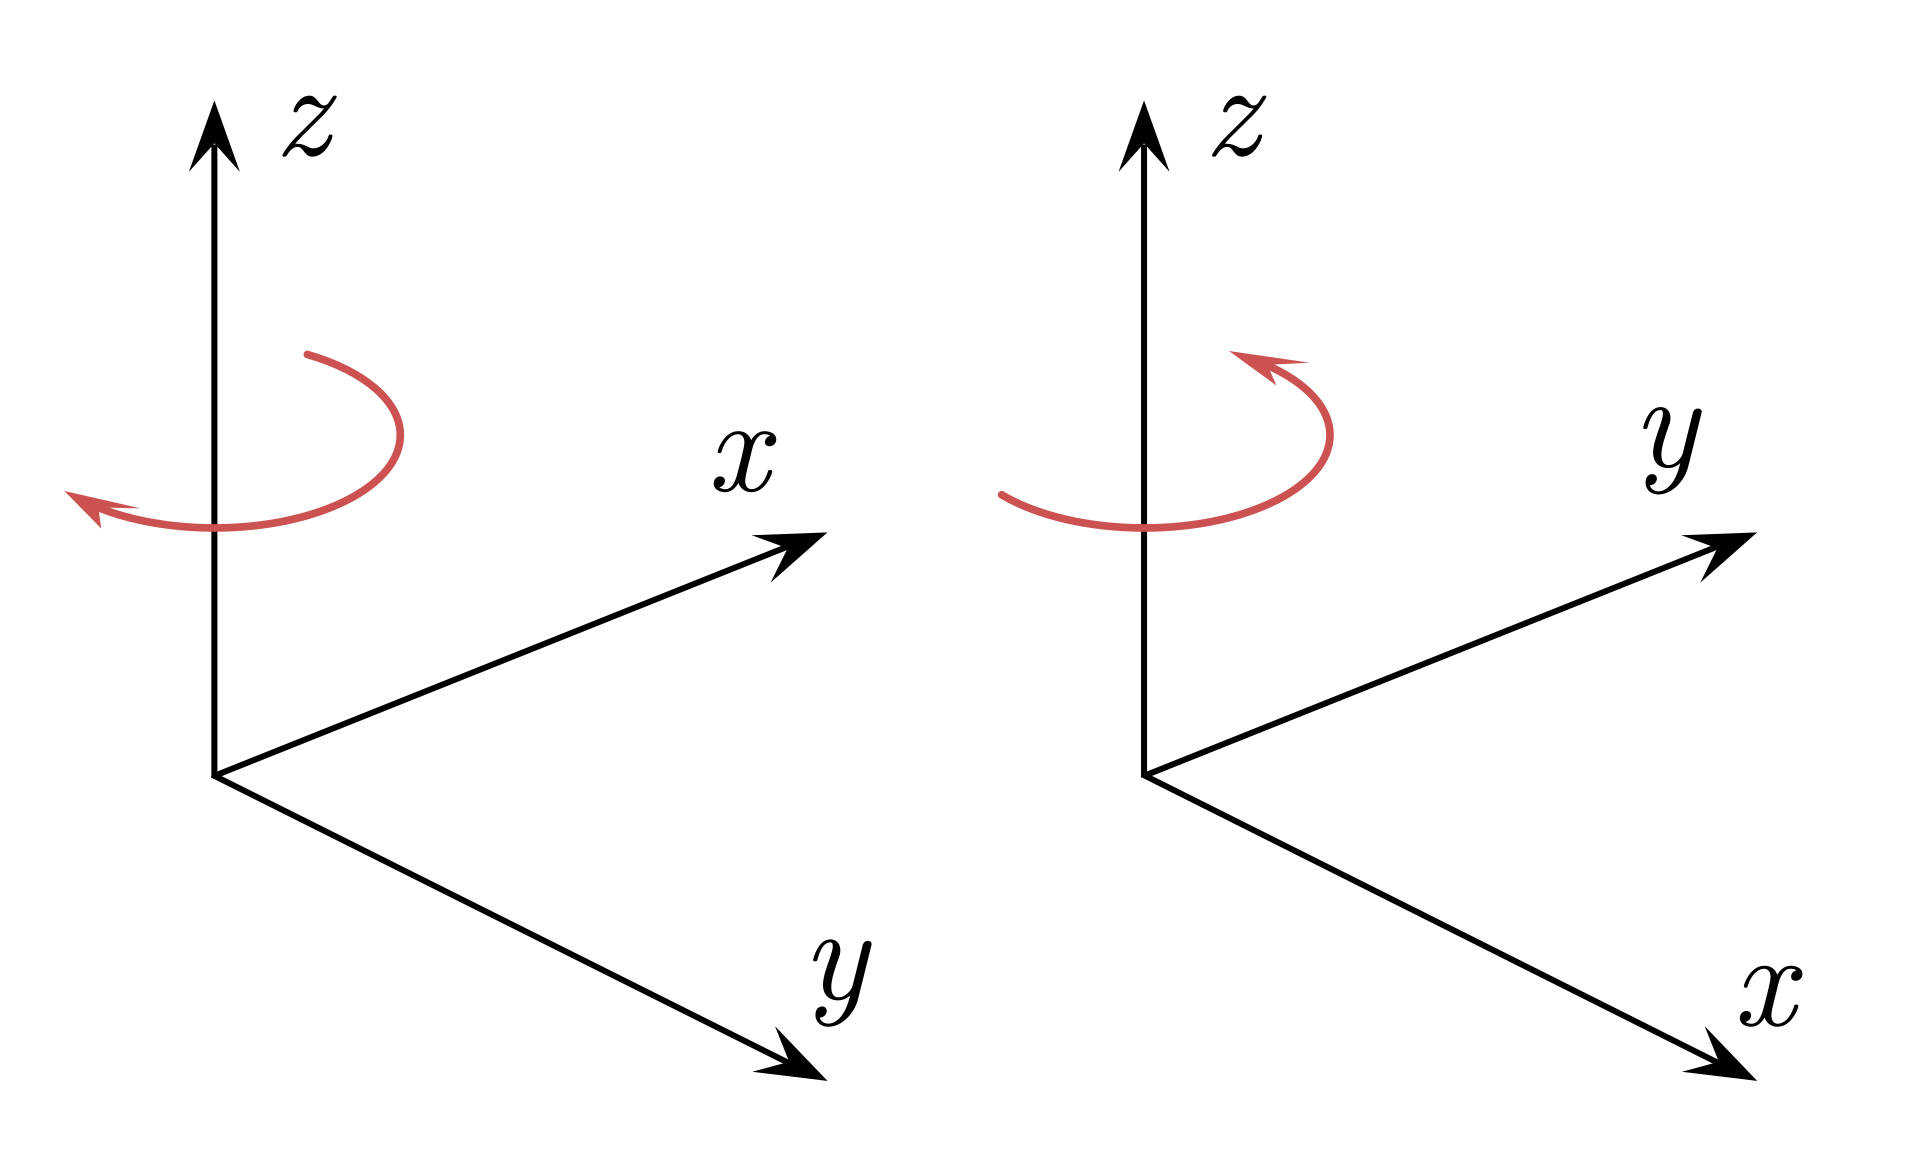
\includegraphics[width=0.5\textwidth]{assets/axis-orientation.png}
	\caption{Левая (слева) и правая (справа) системы координат}
	\label{fig:axis-orientation}
\end{figure}

\textbf{Ориентация системы координат.} (рис. \ref{fig:axis-orientation}) Здесь COLMAP и Blender не отличаются: обе используют правую систему координат, однако интересно упомянуть, что левую также используют в индустрии: например Unity и Unreal Engine.

\textbf{Положение системы координат.} То есть какая ось при открытии софта направлена вверх (по стандарту). В Blender это $+Z$, в COLMAP: $-Y$, в Unity: $+Y$. На математику это никак не влияет, потому что конечному пользователю можно повернуть камеру как удобно, однако это используется как стандартное соглашение по которому камеру разворачивают таким образом, чтобы верх камеры был сонаправлен с этим верхом мировой системы координат.

\begin{figure}[htbp]
	\centering
	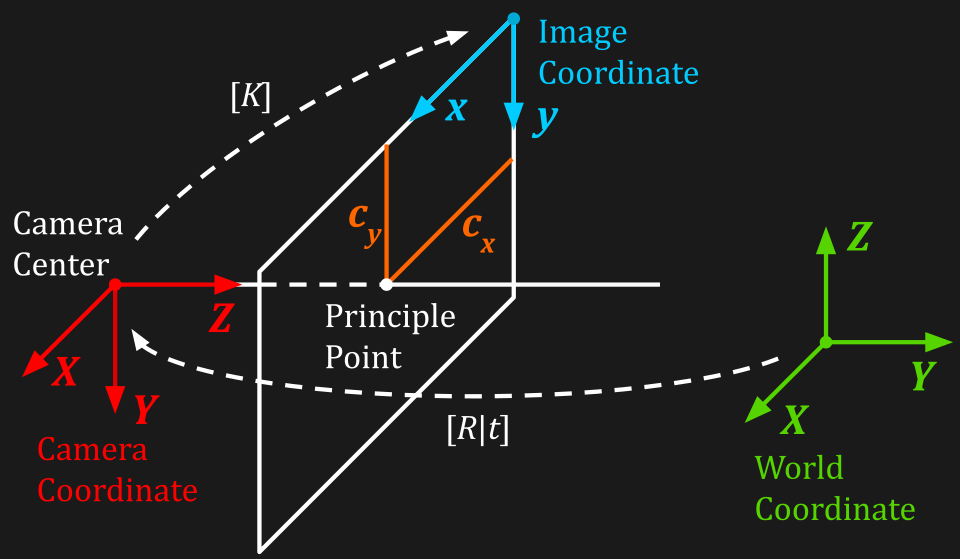
\includegraphics[width=0.5\textwidth]{assets/camera-coords.png}
	\caption{Расположение сенсора в локальных координатах камеры по стандарту OpenCV (используемый в COLMAP)}
	\label{fig:camera-coords}
\end{figure}

\textbf{Оси камеры.} (рис. \ref{fig:camera-coords}) В графике выделяют 3 системы координат: локальные, в текущем изложении не рассматриваются; мировые, отвечают за расположение всех объектов на сцене; видовые, ведут свой отсчет от центра камеры. Видовым координатам соответствуют некоторые локальные оси, в которых принято говорить о направлении взгляда у камеры, то есть с какой стороны и с какой ориентацией расположен сенсор. Отличие между Blender и COLMAP приведено в таблице \ref{tab:colmap_blender_cameras}.

\begin{table}[htbp]
	\centering
	\begin{tabular}{|c|c|c|c|}
		\hline
		& $X$ & $Y$ & $Z$ \\
		\hline
		\textbf{Blender} & Вправо & Вверх & Назад \\
		\hline
		\textbf{Colmap} & Вправо & Вниз & Вперед \\
		\hline
	\end{tabular}
	\caption{Спецификация структуры файла \texttt{cameras.bin}}
	\label{tab:colmap_blender_cameras}
\end{table}

\noindent COLMAP генерирует директорию следующего содержания:

\noindent
\dirtree{%
.1 images/.
.1 sparse/.
.2 0/.
.3 cameras.bin.
.3 images.bin.
.3 points3D.bin.
}

\begin{table}[htbp]
	\centering
	\begin{tabularx}{\textwidth}{llcX}
		\toprule
		\textbf{Поле / Сегмент} & \textbf{Тип данных} & \textbf{Размер (байт)} & \textbf{Описание} \\
		\midrule
		\multicolumn{4}{l}{\textit{Заголовок (Header)}} \\
		\quad num\_cameras & uint64\_t & 8 & Общее количество камер в файле \\
		\midrule
		\multicolumn{4}{l}{\textit{Блок камеры (повторяется num\_cameras раз)}} \\
		\quad camera\_id & int32\_t & 4 & Уникальный ID камеры \\
		\quad model\_id & int32\_t & 4 & ID математической модели камеры \\
		\quad width & uint64\_t & 8 & Ширина изображения в пикселях \\
		\quad height & uint64\_t & 8 & Высота изображения в пикселях \\
		\quad params & double[] & $8 \times N$ & Параметры модели (кол-во $N$ зависит от model\_id) \\
		\bottomrule
	\end{tabularx}
	\caption{Спецификация структуры файла \texttt{cameras.bin}}
	\label{tab:cameras_bin}
\end{table}

\begin{table}[htbp]
	\centering
	\begin{tabularx}{\textwidth}{llcX}
		\toprule
		\textbf{Поле / Сегмент} & \textbf{Тип данных} & \textbf{Размер (байт)} & \textbf{Описание} \\
		\midrule
		\multicolumn{4}{l}{\textit{Заголовок (Header)}} \\
		\quad num\_reg\_images & uint64\_t & 8 & Количество зарегистрированных кадров \\
		\midrule
		\multicolumn{4}{l}{\textit{Блок кадра (повторяется num\_reg\_images раз)}} \\
		\quad image\_id & int32\_t & 4 & Уникальный ID кадра \\
		\quad qvec & double[4] & 32 & Кватернион $[q_w, q_x, q_y, q_z]$ для матрицы $T_\text{w2c}$ \\
		\quad tvec & double[3] & 24 & Вектор трансляции $[t_x, t_y, t_z]$ для матрицы $T_\text{w2c}$ \\
		\quad camera\_id & int32\_t & 4 & ID камеры, которой сделан снимок \\
		\quad image\_name & char[] & Переменный & Имя файла (строка ASCII), завершается \textbackslash x00 \\
		\quad num\_points2D & uint64\_t & 8 & Количество 2D-точек на этом кадре \\
		\midrule
		\multicolumn{4}{l}{\textit{Список 2D-точек кадра (повторяется num\_points2D раз)}} \\
		\quad x & double & 8 & Координата x на изображении (в пикселях) \\
		\quad y & double & 8 & Координата y на изображении (в пикселях) \\
		\quad point3D\_id & int64\_t & 8 & ID 3D-точки (или -1, если связь отсутствует) \\
		\bottomrule
	\end{tabularx}
	\caption{Спецификация структуры файла \texttt{images.bin}. После блока image\_name пайплайн 3DGS его не читает.}
	\label{tab:images_bin}
\end{table}

\begin{table}[htbp]
	\centering
	\begin{tabularx}{\textwidth}{llcX}
		\toprule
		\textbf{Поле / Сегмент} & \textbf{Тип данных} & \textbf{Размер (байт)} & \textbf{Описание} \\
		\midrule
		\multicolumn{4}{l}{\textit{Заголовок (Header)}} \\
		\quad num\_points & uint64\_t & 8 & Количество 3D-точек в облаке \\
		\midrule
		\multicolumn{4}{l}{\textit{Блок 3D-точки (повторяется num\_points раз)}} \\
		\quad point3D\_id & uint64\_t & 8 & Уникальный ID 3D-точки \\
		\quad xyz & double[3] & 24 & Координаты точки в пространстве $[X, Y, Z]$ \\
		\quad rgb & uint8\_t[3] & 3 & Цвет точки в формате $[R, G, B]$ \\
		\quad error & double & 8 & Средняя погрешность репроекции (в пикселях) \\
		\quad track\_length & uint64\_t & 8 & Кол-во кадров, на которых видна эта точка \\
		\midrule
		\multicolumn{4}{l}{\textit{Элементы трека (повторяется track\_length раз)}} \\
		\quad image\_id & int32\_t & 4 & ID кадра, на котором видна точка \\
		\quad point2D\_idx & int32\_t & 4 & Индекс 2D-точки внутри списка points2D этого кадра \\
		\bottomrule
	\end{tabularx}
	\caption{Спецификация структуры файла \texttt{points3D.bin}. Блоки error и track\_length пайплайном 3DGS игнорируются.}
	\label{tab:points3d_bin}
\end{table}

В файле \texttt{cameras.bin} (таблица \ref{tab:cameras_bin}) интересна только камера обскура (pinhole), так как именно она использовалась при рендере изображений. Параметры, которые нужны для её задания следующие: $\mathbf{f_x, f_y}$ --- сколько пикселей по горизонтали и вертикали соответственно умещается в фокусном расстоянии между центром камеры и сенсором; $\mathbf{c_x, c_y}$ --- координаты оптического центра (то есть в какую точку попадает прямая, проведенная из центра камеры перпендикулярно сенсору). Эти данные используются, чтобы перевести точку $(x, y, z)^t$ в координаты пикселя $(u, v)^t$, в который она спроецируется:
%
\[
s \begin{pmatrix} u \\ v \\ 1 \end{pmatrix} =
\begin{pmatrix}
	f_x & 0 & c_x \\
	0 & f_y & c_y \\
	0 & 0 & 1
\end{pmatrix}
\begin{pmatrix} x \\ y \\ z \end{pmatrix}
\]
%

В файл \texttt{images.bin} (таблица \ref{tab:images_bin}) не записывается никакая информация о 2D точках (так как инструментами 3DGS они не считываются). Кватернион вращения и вектор трансляции используется для формирования матрицы $T_\text{w2c}$ 4-го порядка, она используется чтобы переводить мировые однородные координаты в однородные координаты камеры по формуле:
%
\[
	P_\text{camera} = T_\text{w2c} P_\text{world}.
\]
%
Она находится в отношении $T_\text{w2c} = T^{-1}_\text{c2w}$, последняя в свою очередь --- это матрица перевода из координат камеры в мировые. Если подставить точку $(0, 0, 0, 1)^t$, то она должна встать на место центра камеры в мировых координатах, а если единичных вектор направления взгляда, то он повернется так, как повернута камера, откуда следует, что её (камеры) расположение в мировых координатах описывает именно эта матрица.

Значит, чтобы описать матрицу $T_\text{w2c}$ в COLMAP из матрицы $T'_\text{c2w}$ (Blender), можно использовать формулу:
%
\[
	T_\text{w2c} = \left[
		T'_\text{c2w}
		\begin{pmatrix}
			1 & 0 & 0 & 0 \\
			0 & -1 & 0 & 0 \\
			0 & 0 & -1 & 0 \\
			0 & 0 & 0 & 1
		\end{pmatrix}
	\right]^{-1},
\]
%
где диагональная матрица развернёт оси $Y$ и $Z$ в противоположное направление, а в силу того, что её определитель больше нуля, это не ломает ориентацию осей, а затем будет применено исходное перемещение матрицы. В Blender такая камера отличается от исходной поворотом на $\pi$ вокруг локальной оси $X$.

Последний файл --- \texttt{points3D.bin} (таблица \ref{tab:points3d_bin}) --- не представляет из себя ничего особенного. В качестве точек выступают воксели (случайно выбран 1 миллион вокселей), к которым надо применить преобразования, согласованные с тем, что было сделано в Blender. Под это написан скрипт, приведенный в листинге \ref{lst:numpy-to-points3dbin}.